\documentclass[10pt,twocolumn,a4j]{jarticle}
\usepackage{bm}
\usepackage{siunitx}
\usepackage{cases}
\usepackage[japanese]{babel}
\usepackage[dvipdfmx]{graphicx}
\usepackage{subfig}
\columnsep 3zw
\usepackage[dvipdfmx]{graphicx}
\usepackage{subfig} 
\title{A~Computational~Model~of~Cell~Migration~of~Fish~Keratocytes}
\author{生体情報システム研究~~徳永~優}
\date{}
\begin{document}
\maketitle
\section{はじめに}
\begin{figure}[tbp]
\centering
\includegraphics[width=4cm]{kera.eps}
\caption{細胞遊走中のケラトサイト。(撮影:中田多可子氏(岩楯研究室))}
\label{fig:kera}
\end{figure}
魚類表皮細胞ケラトサイトは通常時には円形状であるが、細胞遊走時には半月状の形態に変形し(図\ref{fig:kera})、その形態を維持した状態で移動する。この現象は、細胞の変形がケラトサイトの細胞遊走を実現するために重要な特徴であることを示唆している。しかし、半月状形態がどのようなメカニズムにより形成され、維持されるのかは明らかになっていない。本研究の目的は、ケラトサイトが半月状形態を形成、維持する細胞内メカニズムを物理シミュレーション実験により解明することである。
\section{ケラトサイトの細胞遊走}
ケラトサイトが細胞遊走を行う際、細胞骨格であるアクチン分子が重合してFilamentous actin~(F-actin)を形成することによって細胞膜の方向へ伸長することが報告されており、これが細胞膜の変形および細胞の推進のための原動力になることが示唆されてきた\cite{svitkina1997analysis}。アクチン分子の重合には極性があり、F-actinの一定の端でしか起こらない。アクチン分子は、細胞の前方に多く集中しており、アクチン分子濃度が高い場所であるほど重合の効率が良い\cite{yumura1998spatiotemporal}。重合が起こらない端では逆に、F-actinからアクチン分子が解離していく脱重合が起こっている。また、細胞後部には左右に広がるストレスファイバー(SF)が細胞遊走時には形成されるが、細胞内のアクチン分子を引き戻すアクチンレトログレードフロー(ARF)も報告されている\cite{nakashima2015molecular}。ARFに関して、SFの方向へアクチン分子が引き戻される時に、アクチン分子の重合方向が調整される配向効果も報告されている\cite{swaminathan2017actin}。
\section{シミュレーション手法}
\begin{figure}[tbp]
\centering
 \subfloat[]{%
  \begin{tabular}{c}
   \includegraphics[width=4cm]{top.eps} 
  \end{tabular}
 }%
 \subfloat[]{%
  \begin{tabular}{c}
   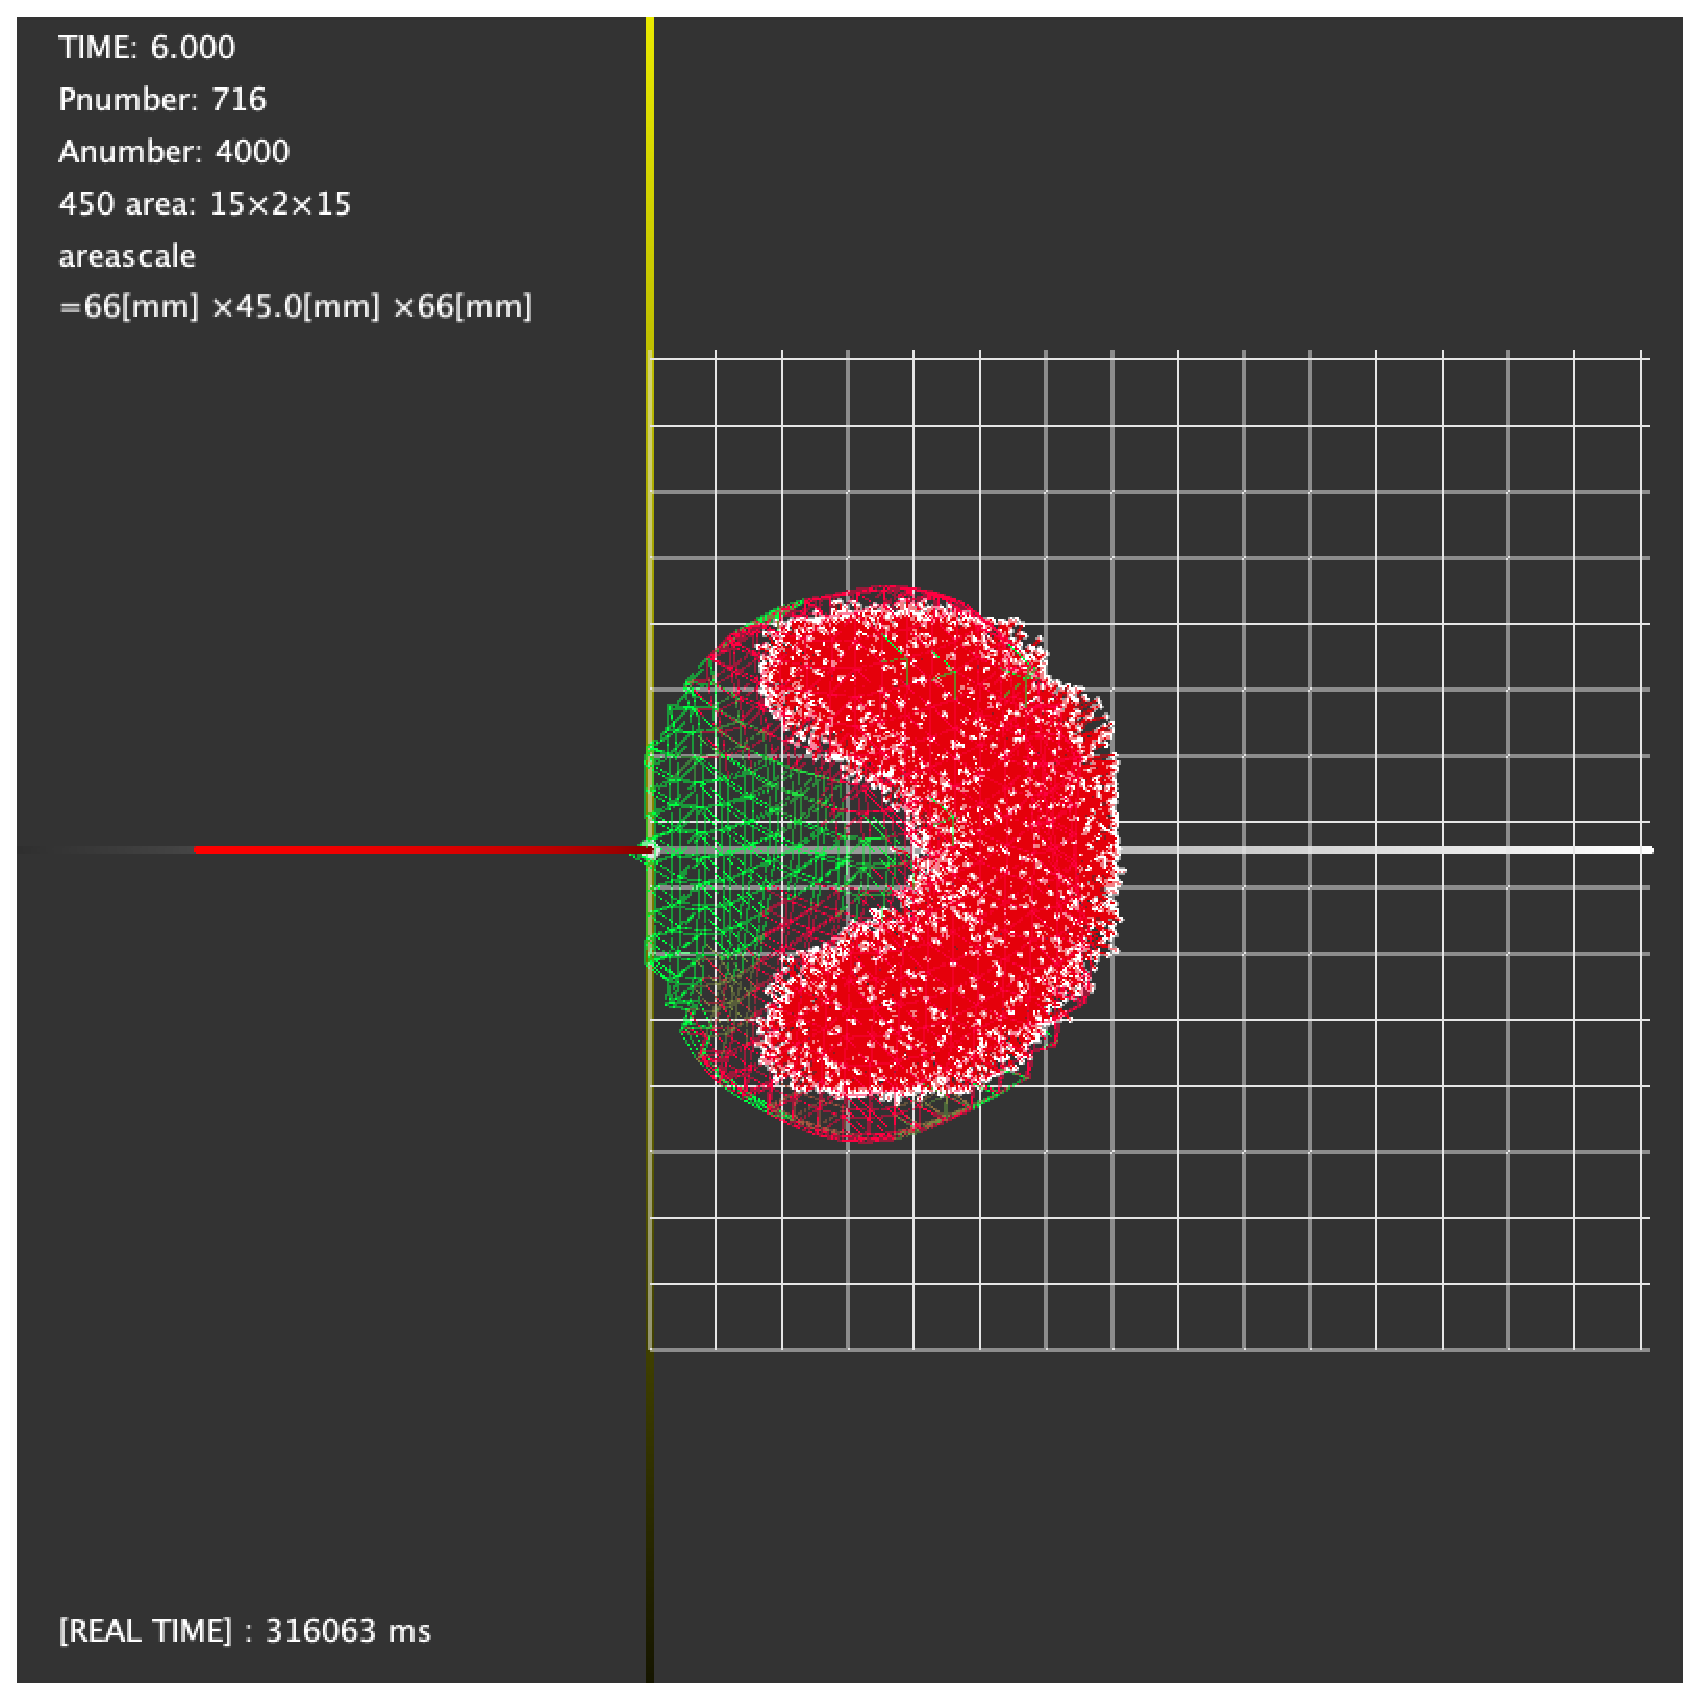
\includegraphics[width=4cm]{top60_arf.eps} 
  \end{tabular}
 }%
 \caption{シミュレーション結果。緑は細胞膜、白は重合前のアクチン分子、赤は重合後のF-actinを示す。(a)~初期配置。膜分子は円柱の表面上、アクチン分子はU字型領域に配置されている。(b)~$t=6.0$でのシミュレーション結果。アクチン分子が半月状に近い形態に凝集している。}
 \label{fig:res0}
\end{figure}
本研究のシミュレーションでは、細胞膜は互いに相互作用する単純な粒子のネットワークによってモデル化し、初期条件として円柱形の表面に配置した。細胞膜の各粒子は以下の運動方程式に従って運動すると仮定した。
\begin{equation}
m\frac{d^2\bm{x}_i}{dt^2} = \bm{F}^m_i +  \bm{F}^a_i - \eta \frac{d\bm{x}_i}{dt}
\end{equation}
ここで、$\bm{x}_i$は膜分子の位置、$\bm{F}^m_i$と$\bm{F}^a_i$はそれぞれ近傍の膜分子から受ける弾性力とF-actinから受ける反発力、$\eta$は粘性抵抗抵抗係数であり、各変数の添え字$i$は第$i$粒子に対する値であることを示す。

アクチン分子は直線上の棒により表現し、重合および解重合はその一端の確率的伸長゙および他端の収縮によってそれぞれ表現した。初期状態において、アクチン分子は長さがなく、各分子のアクチン重合の方向はランダムに決定され、U字型の領域にランダムに配置した。細胞後部の1/5の位置に左右に拡がるSFを仮定し、アクチン分子は確率的にそのSF両端の二点に向かって移動することでARFを近似的に表現した。ARFの効果として、アクチン分子を引く時に重合方向をARFの向きに近づけるようなF-actinの回転を仮定した。全てのアクチン分子重合の方向は初期状態においてランダムに決定されるため、アクチン分子が細胞の上部や下部に伸長して細胞膜へ飛び出してしまうケースがある。そのような場合のために、ある条件に当てはまったアクチン分子を然るべき位置へ移動させる条件を設定する必要がある。

まず、シミュレーション空間のケラトサイトが接着している面を格子状に分割したエリアを作成する。そして、その分割したエリアごとにアクチン分子の密度を計算し、その値が設定された閾値以下であった場合、その該当するエリアに存在するアクチン分子を全て消滅させ、細胞膜の近くに新たに発生させて再びランダムな方向へ重合させる。
\section{結果と考察}
シミュレーション実験の結果、アクチン分子は半月状に凝集することが確認できた(図\ref{fig:res0})。ARFの発生源の位置をSFからずらした場所に設定したり、もしくはARFがアクチン分子を引き戻す強さを弱めたりなど諸条件を変更すると、凝集したアクチン分子の分布が半月状の形状から遠ざかった。ARFの発生源をずらすということはアクチン分子がどの地点に向かって移動するのか、重合方向の回転の大きさが変わることになる。また、ARFを無くした場合ではアクチン分子が細胞膜が反応できずに細胞膜を突き出た。つまり、アクチン分子重合の方向調整をARFの方向と整列させることが半月形の形成に重要であり、そしてARFによるアクチン分子の凝集サイズ収縮を維持することが細胞膜の過度の拡大を防ぐことが示唆された。しかし、ARFが引っ張る方向を変えたり、引き戻す力の大きさを弱めたりなどすると、アクチン分子の凝集形態は半月状から遠ざかった。


\bibliographystyle{junsrt}
\begin{thebibliography}{9}
 \bibitem{yumura1998spatiotemporal} S. Yumura, et al.
    ``Spatiotemporal dynamics of actin concentration during cytokinesis and locomotion in Dictyostelium''  \sl{J. Cell Bio.}\bf{111}\rm{(15)}, 2097-2108, 1998.
     \bibitem{svitkina1997analysis} T. M. Svitkina, et al.
    ``Analysis of the actin--myosin Ⅱ system in fish epidermal keratocytes: mechanism of cell body translocation''  \sl{J. Cell Bio.} \bf{139}\rm{(2)}, 397-415, 1997.
  \bibitem{nakashima2015molecular} H. Nakashima, et al.
    ``The molecular dynamics of crawling migration in microtubule-disrupted keratocytes''  \sl{Bio. and Phy.} \bf{12}\rm{}, 21-29, 2015.
       \bibitem{swaminathan2017actin} V. Swaminathan, et al.
    ``Actin retrograde flow actively aligns and orients ligand-engaged integrins in focal adhesions''  \sl{Proc. Nat. Acad. Sci.} \bf{114}\rm{(40)}, 10648-10653, 2017.
\end{thebibliography}

\end{document}
